\chapter{Proposed human-centered framework}

The fundamental goal of this research is to develop a human-centered framework
for interactive evolutionary computation (IEC) in order to increase users\'
participation and also to minimize the amount of evaluations needed for the
evolutionary process in given Web-based IEC application.

In this chapter an explanation of the proposed framework is described. The
different techniques used, such as user modeling, fuzzy logic, and human-
interaction.

This framework is presented in figure \ref{fig:uc_framework}. Each of the
entities of this framework will be explained in detail in following sections.

\begin{figure*}
	\captionsetup{justification=centering,margin=2cm}
	\centering
	\setlength\fboxsep{0pt}
	\setlength\fboxrule{0.7pt}
	\fbox{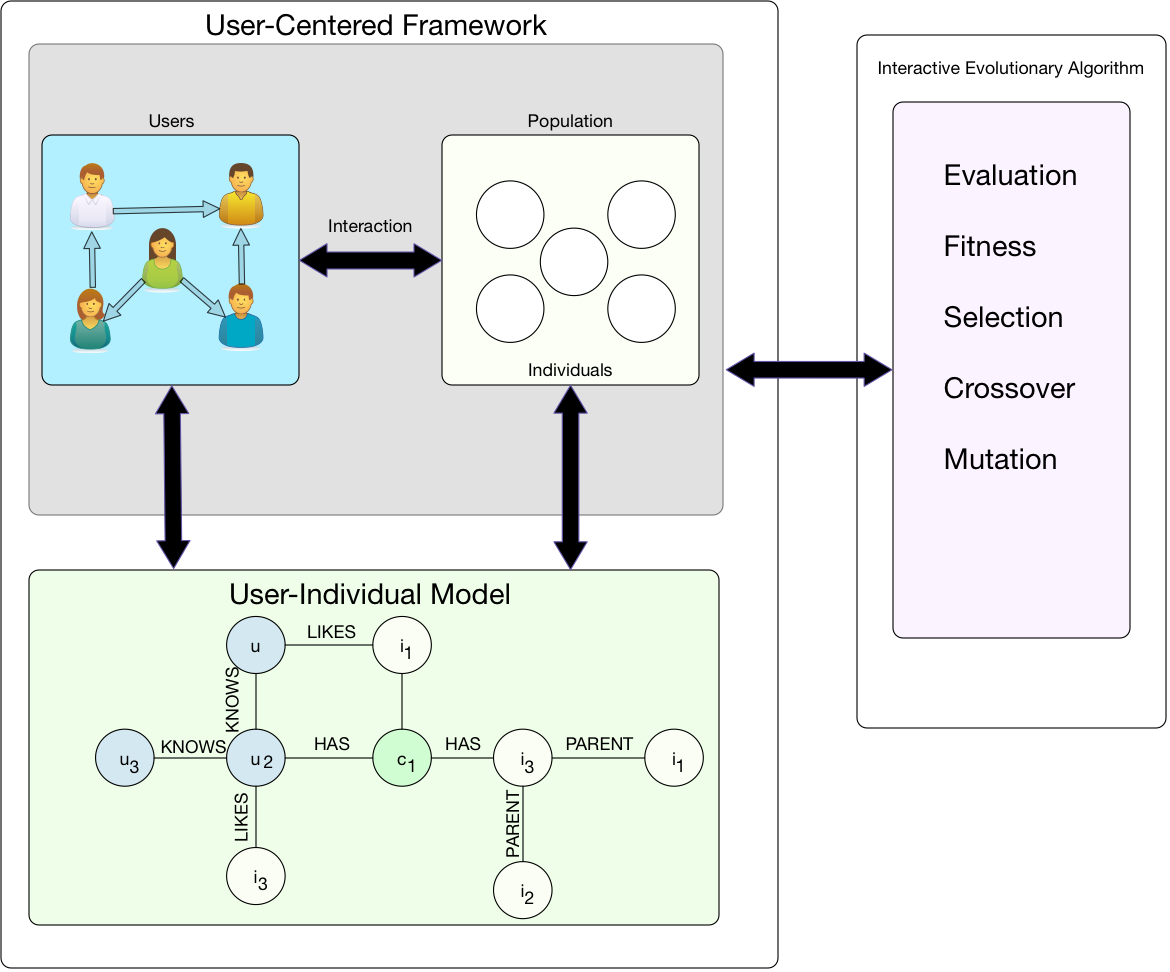
\includegraphics[width=10cm,height=10cm,keepaspectratio]{img/framework.png}}
	\caption{User-Centerd Framework.}
	\label{fig:uc_framework}
\end{figure*}

\section{Users}

Users are a central part of this proposed framework as it aims to study their
behavior when interacting
with individuals or phenotypes within interactive evolutionary
algorithms and other tasks that may exist within IEC systems. Thus users in this
proposal are entities interacting with an evolutionary computation that has the
fundamental purpose of evaluating individuals of a population replacing the
fitness function according to their preferences and mood, among others
\cite{takagi1998interactive}. This form of evaluate individual is given a
subjectively way.

On the other hand in order to capture the attention of users and possibly
increase their participation, currently there exist some basic actions that
users can perform in a given system, going from to be able to access a system
through login mechanism, once the user has logged-in in to the system the users
can interact with different actions, for example the inviting action is when
users can be invited through social networks or maybe from person to person.
Another example is the sharing action that can occur when users want to share
something of their interest through their social networks. In this sense the
action of posting is when users want to put something on their wall.
Likewise the storing action occurs
when users want to retain permanently information that are of their interest.
Finally the browsing action occurs when users are exploring content for their
needs. All these actions go beyond only evaluating individuals.

\begin{figure*}
	\captionsetup{justification=centering,margin=2cm}
	\centering
	\setlength\fboxsep{0pt}
	\setlength\fboxrule{0.7pt}
	\fbox{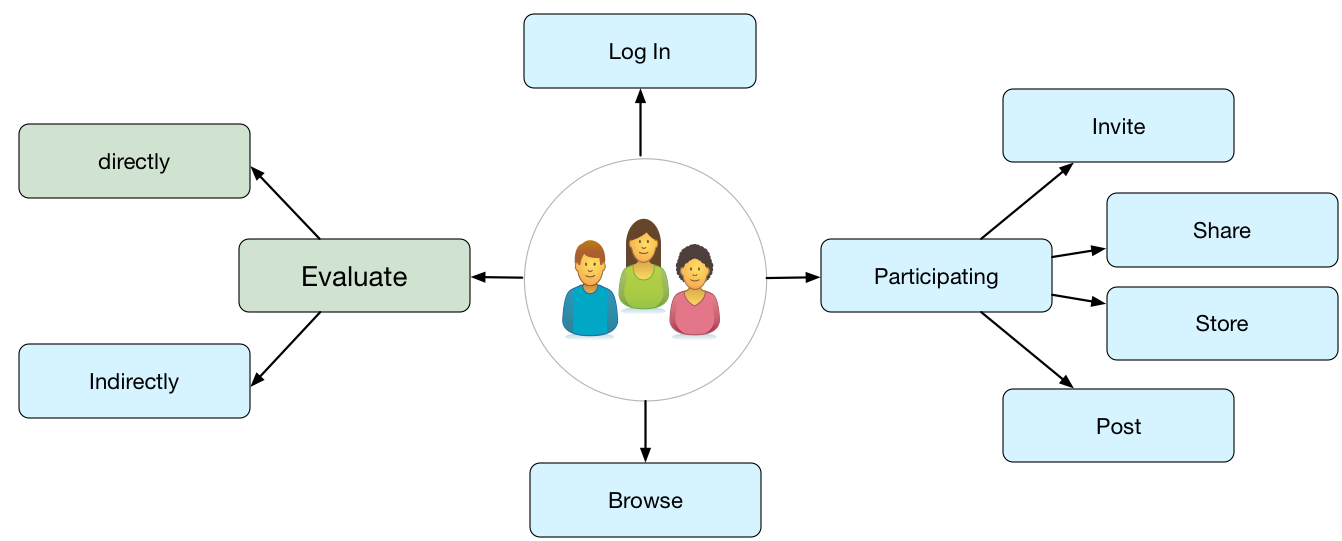
\includegraphics[width=10cm,height=10cm,keepaspectratio]{img/users.png}}
	\caption{Users actions on interactive evolutionary systems.}
	\label{fig:users}
\end{figure*}

In order to start the task of evaluating individuals is necessary that users
access the system through a login mechanism. This mechanism consists of
providing a username and a password in order to grant access to the system. All
users accessing in this way they are considered active users within an IEC
system.

For the evaluating action is proposed that users evaluate individuals
indirectly, this means users can evaluate accepting indirect recommendations of
friends that are currently active in the system. These recommendations can be
store individuals in the system of users who know each other.

Also the browsing action is proposed within IEC systems, this means that users
can explore information that other active users in the system are generating.

Finally the participation activity is proposed. This can be divided into four
different actions as follows:


\begin{itemize}
\item The Inviting action occurs when a user invites another to the system through social networks or from person to person.
\item The sharing action occurs when users share their individual creations with others active users in the system.
\item The posting action occurs when published what they are doing within the system.
\item The storing action occurs when users keep individuals in a collection, the collections concept will be discussed later in this chapter.
\end{itemize}

All the mention above is shown in figure \ref{fig:users}

\section{Individual}

Individuals or phenotypes are entities that form the population for the evolutionary
algorithm. In particular for this work the genotype of individuals
are animated digital
paintings, every individual's phenotype in the population is defined by a chromosome.
This chromosome defines the behavior of the individual, so that it consists of a
vector of real numbers of fifteen genes, where each gen define a particular
behavior in the painting. This individuals combined each other to generated new
individual in the population following the genetic operators such as selection,
crossover and mutation. An example of a individual in this case it is
illustrated in figure \ref{fig:individual}



\begin{figure*}
\captionsetup{justification=centering,margin=2cm}
\centering
\setlength\fboxsep{0pt}
\setlength\fboxrule{0.7pt}
\fbox{\includegraphics[width=10cm,height=10cm,keepaspectratio]{img/individual.png}}
\caption{Individual representation.}
\label{fig:graph}
\end{figure*}


\section{User Model}
Now that both, users an individuals have been defined we can
model the users behavior have with respect to individuals in a graph-based user
model.

The reason for using a graph to model the user-individual is because it
can express in a simple way the behavior of these two entities.
for example a vertex user and individual vertex connected through a edge
representing the semantics of the relationship
as Figure \ref{fig:User-Individual} shows. Each of these vertices contain
properties as well as the edges do; these properties will be explained as follows.

\begin{figure*}
\captionsetup{justification=centering,margin=2cm}
\centering
\setlength\fboxsep{0pt}
\setlength\fboxrule{0.7pt}
\fbox{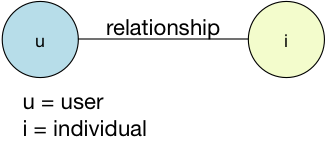
\includegraphics[width=5cm,height=5cm,keepaspectratio]{img/user_individual.png}}
\caption{User-Individual.}
\label{fig:User-Individual}
\end{figure*}

In this proposed graph-based user-individual model the vertices are represented
by a set of vertices or nodes of USERS, INDIVIDUALS, and COLLECTIONS.
The edges are defined by a set of relationships as LIKES,
KNOWS, PARENT, HAS that represents the relationships between the vertices
as seen in figure \ref{fig:User-Individual}.

%Where was this explained?
We already explained the meaning of USERS and INDIVIDUALS, now an explanation is
given for the concept of COLLECTIONS.

In this proposal, a collection is defined as a container where users can
store selected individuals (paintings) laid within the collection. A collection
is created when the user wants to permanently store individuals.

Now the edges in this proposal are explained:

\begin{itemize}
\item The  LIKES edge represents a preference relationship that
a user has with respect to an individual.
\item The  PARENT edge represents an ancestor of an individual,
 in other words where the individual comes from.
\item Likewise the HAS edge represents that certain user has a collection.
\item Finally the KNOWS edge represents a relationship of friendship between users
and is established by their social network.
\end{itemize}

The above mentioned is illustrated by Figure~\ref{fig:Nodes_Edges}.

\begin{figure*}
\captionsetup{justification=centering,margin=2cm}
\centering
\setlength\fboxsep{0pt}
\setlength\fboxrule{0.7pt}
\fbox{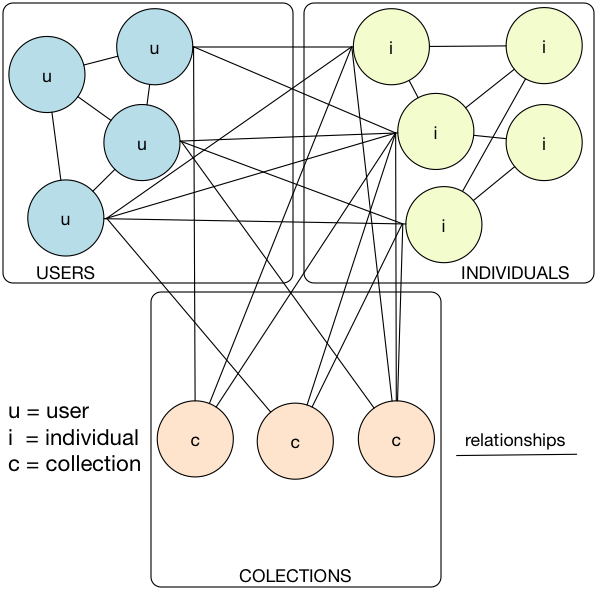
\includegraphics[width=10cm,height=10cm,keepaspectratio]{img/user_individual_collections.png}}
\caption{Nodes And Edges Representation.}
\label{fig:Nodes_Edges}
\end{figure*}


In each vertex is necessary to store knowledge about users, individuals and
also for the collections, this is known as a property.

It is worth to mention that all vertices have a property called “element\_type”
among others. This property is used to identify which type of vertex is, for
example if vertex corresponds to a user then this property labels the vertex as a
“person” type. Likewise if the vertex corresponds to an individual this property
labels it as an “individual” and is the same for any vertex we want to add to the
model. This property also has the purpose of being able to do operations on the
graph according to the vertex type.

The properties for the vertex “u” are the following:

\begin{itemize}
\item id.
\item created.
\item name.
\item element\_type.
\end{itemize}

The “id” property defines that the vertex u has a unique identifier in the set
of vertices, which means that there will not be duplicate vertices. The property
“created” defines the creation date of the vertex $u$. The property “name”
defines the name of the vertex u. The property “element\_type” defines the
element type that will be the vertex $u$.

In figure \ref{fig:User_node} the vertex $u$ properties are shown.

\begin{figure*}
\captionsetup{justification=centering,margin=2cm}
\centering
\setlength\fboxsep{0pt}
\setlength\fboxrule{0.7pt}
\fbox{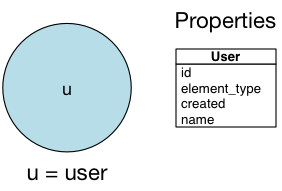
\includegraphics[width=5cm,height=5cm,keepaspectratio]{img/user_node.png}}
\caption{User Properties.}
\label{fig:User_node}
\end{figure*}

The properties for the vertex $i$ are the following:
\begin{itemize}
\item id.
\item created.
\item element\_type.
\item chromosome.
\item views.
\end{itemize}

The “id” property defines that the vertex $i$ has a unique identifier in the set
of vertices, which means that there will not be duplicate vertices. The
“chromosome” property defines the chromosome of the individual representing the
vertex $i$. which as defined above in this section. The property “views” defines
the amount that users have seen this vertex $i$ The property “element\_type”
defines the element type that will be the vertex $i$. The property “created”
defines the creation date of the vertex $i$.



In figure \ref{fig:Individual_node} the vertex $i$ properties are shown.

\begin{figure*}
\captionsetup{justification=centering,margin=2cm}
\centering
\setlength\fboxsep{0pt}
\setlength\fboxrule{0.7pt}
\fbox{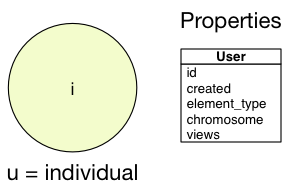
\includegraphics[width=5cm,height=5cm,keepaspectratio]{img/individual_node.png}}
\caption{Individual Properties.}
\label{fig:Individual_node}
\end{figure*}

The properties for the vertex “c” are the following:

\begin{itemize}
\item id.
\item element\_type.
\item created.
\item name.
\end{itemize}

The “id” property defines that the vertex $c$ has a unique identifier in the set
of vertices, which means that there will not be duplicate vertices. The
property “name” defines the name of the vertex $c$. The property “created”
defines the creation date of the vertex $c$.

In figure \ref{fig:Collection_node} the vertex $c$ properties are shown.

\begin{figure*}
\captionsetup{justification=centering,margin=2cm}
\centering
\setlength\fboxsep{0pt}
\setlength\fboxrule{0.7pt}
\fbox{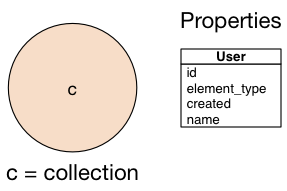
\includegraphics[width=5cm,height=5cm,keepaspectratio]{img/collection_node.png}}
\caption{Collection Properties.}
\label{fig:Collection_node}
\end{figure*}

In the same way that the vertices have properties also the edges, these
properties are defined as follows.

The “LIKES” edge has the following properties:

\begin{itemize}
\item id.
\item created.
\item rate.
\end{itemize}

The “id” property defines that the “LIKES” edge has a unique identifier in the
set of edges, which means that there will not be duplicate edges. The property
“created” defines the date of creation of the this edge. The property “rate”
defines the rate that the users give to the individual store in this edge.

In figure \ref{fig:Likes_edge} the edge “LIKES” properties and the relationships
with the vertices $u$ and $i$ are shown.


\begin{figure*}
\captionsetup{justification=centering,margin=2cm}
\centering
\setlength\fboxsep{0pt}
\setlength\fboxrule{0.7pt}
\fbox{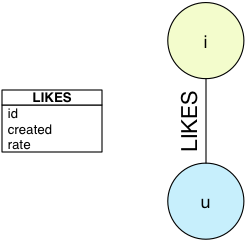
\includegraphics[width=5cm,height=5cm,keepaspectratio]{img/edge_properties_likes.png}}
\caption{LIKES edge Properties.}
\label{fig:Likes_edge}
\end{figure*}

The “KNOWS” edge has the following properties.
\begin{itemize}
\item id.
\item created.
\end{itemize}

The “id” property defines that the edge “KNOWS” has a unique identifier in the
set of edges, which means that there will not be duplicate edges. The property
“created” defines the date of creation of the edge.

In figure \ref{fig:Knows_edge} the edge “KNOWS” properties and the relationships between vertex “u”
are shown.

\begin{figure*}
\captionsetup{justification=centering,margin=2cm}
\centering
\setlength\fboxsep{0pt}
\setlength\fboxrule{0.7pt}
\fbox{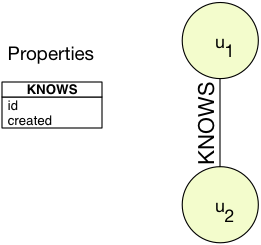
\includegraphics[width=5cm,height=5cm,keepaspectratio]{img/edge_properties_knows.png}}
\caption{KNOWS edge Properties.}
\label{fig:Knows_edge}
\end{figure*}

The “PARENT” edge has the following properties, and represent the parents of a
new individual.
\begin{itemize}
\item id.
\item created.
\end{itemize}

The “id” property defines that the edge “PARENT” has a unique identifier in the
set of edges, which means that there will not be duplicate edges. The property
“created” defines the date of creation of the edge.

In figure \ref{fig:Parent_edge} the edge “PARENT” properties and the
relationship between vertex $i$ are shown.

\begin{figure*}
\captionsetup{justification=centering,margin=2cm}
\centering
\setlength\fboxsep{0pt}
\setlength\fboxrule{0.7pt}
\fbox{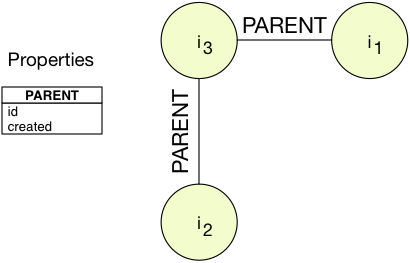
\includegraphics[width=5cm,height=5cm,keepaspectratio]{img/edge_properties_parent.png}}
\caption{PARENT edge Properties.}
\label{fig:Parent_edge}
\end{figure*}

The edge “HAS” has the following properties, and represent the parents of a new individual.
\begin{itemize}
\item id.
\item created.
\end{itemize}

The “id” property defines that the edge “HAS” has a unique identifier in the set
of edges, which means that there will not be duplicate edges. The property
“created” defines the date of creation of the edge.

In figure \ref{fig:Has_edge} the edge “HAS” properties and the relationship
between vertices $u$, $i$ and $c$ are shown.

\begin{figure*}
\captionsetup{justification=centering,margin=2cm}
\centering
\setlength\fboxsep{0pt}
\setlength\fboxrule{0.7pt}
\fbox{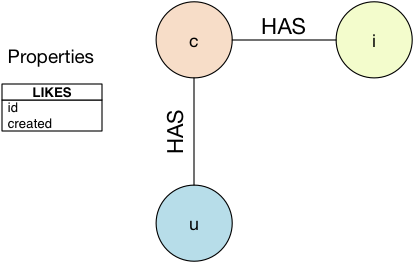
\includegraphics[width=5cm,height=5cm,keepaspectratio]{img/edge_properties_has.png}}
\caption{HAS edge Properties.}
\label{fig:Has_edge}
\end{figure*}

% \begin{equation*}\label{eq:graphRelDef}
% \displaystyle
% \begin{split}
% V &= \{[u_1,u_2,u_3,...,u_n],[i_1,i_2,i_3,...,i_n],[c_1,c_2,c_3,...,c_n]\},\\
% E&= \{[l_1,l_2,l_3,..,l_n],[p_1,p_2,p_3,...,p_n],[h_1,h_2,h_3,...,h_n],[k_1,k_2,k_3,...,k_n]\}\\
% \end{split}
% \end{equation*}

Figure \ref{fig:user_moder} shows an example of the graph-based
user-individual model.

\begin{figure*}
\captionsetup{justification=centering,margin=2cm}
\centering
\setlength\fboxsep{0pt}
\setlength\fboxrule{0.7pt}
\fbox{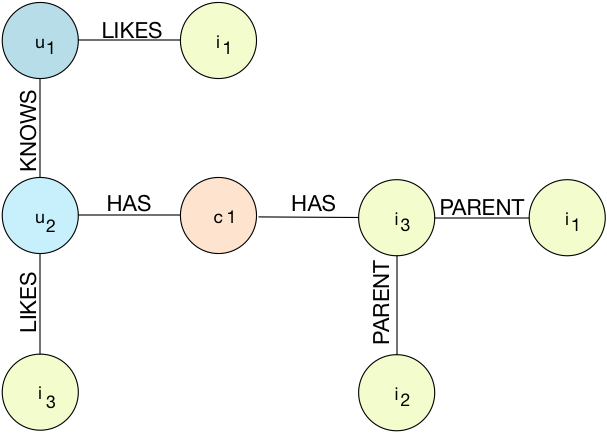
\includegraphics[width=8cm,height=8cm,keepaspectratio]{img/model_representation.png}}
\caption{Graph-based user-individual model.}
\label{fig:user_moder}
\end{figure*}
